

\chapter{Overview TLS}





1.	Rabi Oszillationen

2.	(perturbed) Free induction decay

3.	Ramsey fringes

4.	Double resonance spectroscopy

5.	Frequency modulation / Kador

6.	Quantum beats

7.	Strong coupling 

8.	Pump-probe spectroscopy (?)

9.	2D spectroscopy, Feynman diag.





Wir beginnenn die kohärente Spektroskopie  mit ein paar
Grundlagen (und einem neuen Buch).

\section{8.1. Wdh. Störungsrechnung, Fermis Goldene Regel und
Einstein-Koeffizienten\protect\footnote{Rand, Kap. 3.2 und 3.5}\hfill w} 

Das haben wir schon gemacht. Freunden sie sich mit der
Notation von Stephen Rand an.

\section{8.2. Störungsrechnung vs. Exakte Lösung (Rabi)\protect\footnote{Rand, Kap. 3.3 \newline Hamm 2005, Kap. 1 \newline Christoph Schnupfhagn}\hfill *} 

Verstehen sie die Grenzen der Störungsrechung und den
Unterschied zum exakten Rabi-Formalismus. \footnote{Warum vergleicht Rand das Ergebnis der Störungsrechnung mit Dämpfung mit der Lösung von Rabi ohne Dämpfung? Vergleicht man die Ergebnisse jeweils ohne Dämpfung, sind diese bis auf den Vorfaktor vor der Oszillation sehr ähnlich.}

Mit dem Störungsansatz für den Hamiltonoperator, welcher bereits in Kapitel \ref{sec:stoerungstheorie} eingeführt wurde, lassen sich die Differentialgleichungen für die Zeitentwicklung der Faktoren $C_{1}$ und $C_{2}$ herleiten. In der \emph{rotating wave approximation} (Vernachlässigung der Terme mit $\omega_{0} + \omega$) lauten diese:
\begin{align}
    \dot{C_{2}} & = \frac{i \Omega}{2} e^{i (\omega_{0} - \omega) t} C_{1} - \frac{1}{2} \gamma_{2} C_{2} \label{eq:rabi1} \\
    \dot{C_{1}} & = \frac{i \Omega^{\ast}}{2} e^{-i (\omega_{0} - \omega) t} C_{2} - \frac{1}{2} \gamma_{1} C_{1} \label{eq:rabi2}
\end{align}
Dabei ist $\Omega = \vec{\mu}_{21} \cdot \vec{E}_{0} / \hbar$ und $\omega_{0}$ die Differenzfrequenz der Energieniveaus 1 und 2. Die zweiten Summanden werden jeweils phänomenologisch hinzugefügt, um der spontanen Relaxation der Zustände Rechnung zu tragen. Im Folgenden wird jedoch $\gamma_{1} = \gamma_{2} = 0$ angenommen.

Bisher wurde das obige System zweier Differentialgleichungen für kleine Zeiten genähert. Aufgrund der Anfangsbedingungen $C_{1}(0) = 1$ und $C_{2}(0) = 0$ gilt dann
\begin{align}
    \dot{C_{2}} & = \frac{i \Omega}{2} e^{i (\omega_{0} - \omega) t} C_{1} \\
    \dot{C_{1}} & = 0.
\end{align}
Die Wahrscheinlichkeit, dass sich das Molekül nach der Zeit $t$ im angeregten Zustand befindet, ist dann gegeben durch
\begin{equation}
    \vert C_{2}(t) \vert^{2} = \left[ \frac{\Omega}{2} \frac{\sin((\omega_{0} - \omega) t/2)}{(\omega_{0} - \omega)/2} \right]^{2}
    \label{eq:c2-approx}
\end{equation}
und oszilliert somit in der Zeit. Die Lösung divergiert allerdings für $\omega_{0} \rightarrow \omega$, d.h.\ bei der Resonanz. Da aus Gründen der Normierung immer $\vert C_{2}(t) \vert^{2} \leq 1$ gelten muss, ist diese Lösung nicht physikalisch.

Gleichungen \ref{eq:rabi1} und \ref{eq:rabi2} können jedoch auch exakt gelöst werden für den Fall $\gamma_{1} = \gamma_{2} = 0$, was als Rabi-Formalismus bezeichnet wird. Daraus ergibt sich die Besetzungswahrscheinlichkeit
\begin{equation}
    \vert C_{2}(t) \vert^{2} = \left[ \frac{\Omega}{2} \frac{\sin(\Omega_{R} t/2)}{\Omega_{R}/2} \right]^{2}
\end{equation}
mit der Rabi-Flopping-Frequenz $\Omega_{R} = [ \Delta^{2} + \Omega^{2} ]^{1/2}$ und $\Delta = \omega_{0} - \omega$. $\vert C_{2}(t) \vert^{2}$ ist für den Resonanzfall $\Delta = 0$ in Abbildung \ref{fig:rabi} eingezeichnet. Es ist zu erkennen, dass das Molekül periodisch zwischen angeregtem und Grundzustand wechselt (\emph{Rabi Flopping}) und somit eine periodische Besetzungsinversion erreicht werden kann. Die Lösung von Rabi zeigt keine Divergenz mehr im Vergleich zu Gleichung \ref{eq:c2-approx}.

\begin{figure}
    \centering
    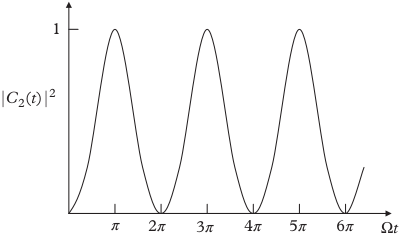
\includegraphics[width = 0.7 \textwidth]{\currfiledir/Rabi.png}
    \caption{Lösung von Rabi im Resonanzfall $\Delta = 0$. Das Molekül wechselt periodisch zwischen angeregtem und Grundzustand.}
    \label{fig:rabi}
\end{figure}

\section{8.3. Dichte-Matrix\protect\footnote{Rand,  Kap. 3.6 \newline Parson, Kap. 10.2 \newline Hamm 2005, Kap. 1}\hfill **} 

Die Dichte-Matrix ist wichtig, um inkohärente Zustände zu
beschreiben, kommt in der QM aber oft zu kurz. \footnote{Warum kann man ein Ensemble von Teilchen nicht durch eine einzelne Wellenfunktion beschreiben, sondern nur durch eine Summe von Dichtematritzen?}
\footnote{Ich habe das so verstanden, dass ein reiner Zustand eine köhärente Superposition einzelner Zustände und damit Wellenfunktionen ist. Hat dieser Begriff der Kohärenz etwas mit dem aus der Optik zu tun?}

\section{8.4. Optische Bloch-Gleichungen\protect\footnote{Rand, Kap. 3.8, Simon Biberger}\hfill ***} 

\textit{Man kann die Wechselwirkung von Licht mit einem
Zwei-Niveau-System auf Kreisel-Physik abbilden.}
\footnote{Was versteht man unter inkohärentem Pumpen?}
\footnote{Was genau kann man sich unter dephasing vorstellen?}
Um den Hermiteschen Charakter des Hamilton-Operators zu erhalten, muss beim Beachten von Zerfallstermen die Bewegungsgleichung folgendermaßen modifiziert werden.
\begin{align}
    i\hbar \dot{\hat{\rho}} =& [\hat{H},\hat{\rho}] + Relaxationsterme \notag\\
    =& [\hat{H},\hat{\rho}] \pm i\hbar\Lambda \pm i\hbar\gamma \hat{\rho} - i\hbar \Gamma \hat{\rho}
\end{align}
Der erste Term berücksichtigt die Abnahme durch inkohärentes Pumpen, der zweite die strahlende und nicht-strahlende Populations-Relaxation. Der letzte beachtet das dephasing. %dem Verlust der genauen Information über die zeitliche Entwicklung der Signale 

Unter bestimmten Bedingungen können die Dichte-Matrix-Bewegungsgleichungen in eine praktische Form übergeführt werden, die als optische Bloch-Gleichungen bekannt sind, welche eine ähnliche Form wie die Kreisel-Präzession besitzen. Die einfachste Form der Bloch-Gleichungen beschreibt ein Zwei-Niveau-System und wird Vektor-Modell genannt.\\

Mithilfe der Rotating-Wave-Approximation (RWA) und der slowly varying envelope approxiamtion (SVEA) erhält man
\begin{align}
    V_{21}=& -\frac{1}{2}\mu_{21}E_0e^{-i\omega t} \label{Bloch1}\\
    \rho_{21} =& \tilde{\rho}_{21}e^{-i\omega t} \label{Bloch2}.
\end{align}
$\tilde{\rho}_{21}$ beschreibt hier die langsam variierende Amplitude des Matrixelemente, welche proportional zur Amplitude der Ladungs-Oszillation bei der bestimmten optischen Frequenz ist.\\
Mit den Gleichungen \ref{Bloch1} und \ref{Bloch2} erhält man für die Zeitentwicklung von $\tilde{\rho}_{21}$:
\begin{equation}
    \left( \frac{d}{dt} + i\Delta + \Gamma\right)\tilde{\rho}_{21}=-\frac{i}{2}\Omega(\rho_{22}-\rho_{11}).
\end{equation}
Dabei gilt $\Delta$= $\omega_0 - \omega$ und $\Omega$ = $\frac{\mu_{21}E_0}{\hbar}$.\\
Damit lassen sich drei Komponenten eines 3-dim. Vektors definieren.
\begin{align}
    R_1 =& \tilde{\rho}_{21} + \tilde{\rho}_{12}  \notag \\
    R_2 =& i(\tilde{\rho}_{21}-\tilde{\rho}_{12})\\
    R_3 =& \rho_{22} -\rho_{11} \notag
 \end{align}
 \begin{equation}
     \bar{R} = R_1\tilde{e}_1 + R_2\tilde{e}_2 + R_3\tilde{e}_3
 \end{equation}
 Für die Zeitentwicklung der drei Komponenten erhält man mit $\Gamma$ = $\frac{1}{T}$:
 \begin{align}
    \dot{R_1} =& -\Delta R_2 - \frac{1}{T}R_1  \notag \\
    \dot{R_2} =& \Delta R_1 - \frac{1}{T}R_2 + \Omega R_3 \label{Bloch3}\\
    \dot{R_3} =& - \frac{1}{T}R_3 - \Omega R_2 \notag
 \end{align}
 Die Gleichungen \ref{Bloch3} werden optische Bloch-Gleichungen genannt. Kompakter lassen sich die drei Gleichungen mit
 \begin{equation}
     \dot{\bar{R}} = -\frac{1}{T}\bar{R} + \bar{\beta} \times \bar{R}
 \end{equation}
schreiben, wobei $\bar{\beta}$ = $\Omega \hat{e}_1$ + $\Delta \hat{e}_3$ ist.\\
Die Bewegung des Bloch-Vektors ist in Abbildung \ref{fig:Bloch} zu sehen. Für die gezeigte Orientierung von $\bar{\beta}$ ist das detuning positiv.
\begin{figure} [h]
    \centering
    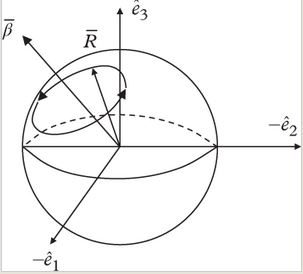
\includegraphics[width = 0.7 \textwidth]{\currfiledir/Bloch.JPG}
    \caption{Präzession des Bloch-Vektors $\bar{R}$ um ein effektives Feld $\bar{\beta}$.}
    \label{fig:Bloch}
\end{figure}
\section{8.5. Polarization und abgestrahlte Felder\protect\footnote{Rand, Kap. 3.9}\hfill **} 

Wie kommt es, dass man am Ende etwas detektieren kann? \footnote{Die Lösung der Wellengleichung liefert ein elektrisches Feld, dessen Betrag proportional zur Länge der Probe ist. Eigentlich sollte dies aber doch das Pendant zum Lambert-Beerschen Gesetz sein, also eher einen exponentiellen Zusammenhang mit der Länge aufweisen?}

\section{8.6. Absorption in der Dichte-Matrix-Darstellung\protect\footnote{XXX ???}\hfill *} 

Das Optische Theorem hilft zu verstehen, warum in einem
Transmissionsexperiment am Ende Licht fehlt, und wie das mit
der Dichtematrix zusammenhängt.



\section{ 9. Effekte der Bloch-Gleichungen / NMR mit Licht} 

Wir betreiben Kreisel-Physik  mit Licht anhand von einigen
klassischen Beispielen

\section{9.1. Rabi-Oszillationen\protect\footnote{Rand, Kap. 4.1, Simon Biberger}\hfill ***} 

\textit{Das Zwei-Niveau-System oszilliert entweder als Funktion der
Zeit oder der 'pulse area' zwischen Grund- und angeregtem
Zustand.}\\
Betrachtet man ein Atom, das plötzlich Licht ausgesetzt ist, welches resonant mit einem Übergang aus dem Grundzustand ist. So kann es zu einem kohärenten transienten Phänomen kommen, der Nutation. Die Nutation beschreibt den Aufbau einer Polarisation, welche durch die Anwesenheit eines optischen Feldes verursacht wird.\\
Da die Rabi-Oszillationen in Bezug auf Populationszerfälle schnelle Prozesse sind, vereinfachen sich die Bloch-Gleichungen zu:
\begin{align}
    \dot{R_1} =& -\Delta R_2  \notag \\
    \dot{R_2} =& \Delta R_1 + \Omega R_3 \label{Rabi}\\
    \dot{R_3} =& - \Omega R_2 \notag
 \end{align}
Diese Gleichungen lassen sich bei Mitnahme eines möglichen Doppler-Shifts ($v_z$) und mit einer Anfangsverteilung der Population $R_3$(0) lösen.
\begin{align}
    R_1(t) =& \frac{\Omega \Delta}{\Omega_R^2}R_3(0)\cdot cos(\Omega_Rt-1) \notag \\
    R_2(t) =& \frac{\Omega}{\Omega_R}R_3(0)\cdot sin(\Omega_Rt) \label{Rabi2}\\
    R_3(t) =& R_3(0)\cdot \left[1+\frac{\Omega^2}{\Omega_R^2}\cdot 
    cos(\Omega_Rt-1)\right] \notag
\end{align}
Dabei ist $\Omega_R^2$ = $\Delta^2 + \Omega^2$, $\Delta = \omega_0-\omega-kv_z$ und $\Omega = \mu_{21}E_{12}/\hbar$.\\
Der Betrag des Bloch-Vektors bleibt über die betrachtete Zeit konstant. Er präzediert um den Vektor $\bar{\beta}$ mit der Frequenz $\Omega_R$.
Für den Resonanzfall $\Delta = 0$ kommt es zum Rabi-flopping. Dabei springt  $\bar{\beta} = \Omega \hat{e}_1$ auf $\bar{\beta} = -\Omega \hat{e}_1$. Das Atom oszilliert also zwischen dem angeregten und Grundzustand unter dem Einfluss eines treibenden Feldes.\\
Die Rabi-Oszillationen können über zwei Methoden gemessen werden. Entweder betrachtet man die Zeitentwicklung der Fluoreszenz bei einem festen treibenden Feld oder die Transmissionsänderung während der Variation der treibenden Feldes.
\begin{figure} [h]
    \centering
    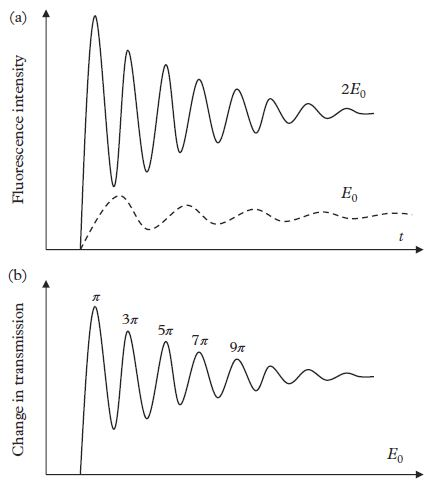
\includegraphics[width = 0.7 \textwidth]{\currfiledir/Rabi1.JPG}
    \caption{Rabi-Oszillationen in (a) transienter Fluoreszenz und (b) differentielle Transmissionsmessung.}
    \label{fig:Rabi}
\end{figure}

\section{9.2. Free Induction Decay\protect\footnote{Rand, Kap. 4.2}\hfill **} 

Nach dem Ausschalten des Lasers wird noch ein Feld
abgestrahlt.

\section{9.3. Photon Echo\protect\footnote{Rand, Kap. 4.3}\hfill ***} 

Mehrere Lichtpulse wechselwirken mit einem inhomogenen
Ensemble von Atomen / Fluorophoren. Nachdem alle Pulse
vorbei sind wird trotzdem noch ein Feld emittiert. Dies ist
eine elegante Methode, um die Inhomogenität eines Ensembles
zum umgehen.
 
 